\documentclass[8pt,a4paper]{extarticle}
%\documentclass[8pt,twocolumn,a4paper]{extarticle}
%\documentclass[6pt,a4paper]{article}
\usepackage[utf8]{inputenc}
\usepackage{amsmath}
\usepackage{amsfonts}
\usepackage{amssymb}
\usepackage{graphicx}
\usepackage{enumitem}
\usepackage{setspace} 
\usepackage{float}
\usepackage{url}
\usepackage[usenames,dvipsnames,svgnames,table]{xcolor}
\usepackage{multicol}

\pagecolor{black}
\setlist{nolistsep}
\topmargin -2cm
\oddsidemargin -1.5cm
\evensidemargin -1.5cm
\textwidth 18.75cm
\textheight 26cm
\linespread{1.00}
\color{YellowOrange}

%Other Colors: ForestGreen,Cerulean,Salmon,Purple, Red, White

\twocolumn
\title{Title Here}
\author{Author Name Here}

\begin{document}

\newcommand{\mitem}{\item[$\square$]}
\newcommand{\mmitem}{\item[$\triangledown$]}

\maketitle


\section*{First React Application:}

\begin{itemize}
\item To start a React Project, most developers will utilize the create-react-app project template (a node package). Simply install this package and run it to start.
Specifically:

\begin{verse}

npx create-react-app <project name>
mkdir <project name>
npm start

\end{verse}

to install and get the local server running.

\item \textbf{Project Structure:}
\item \textbf{./node_modules:} All locally installed node dependences are stored here.
\item \textbf{./public:} index.html (front page, robots.txt and favicons stored here.
\item \textbf{./src:} Contains the React Apps (self-contained pieces of interface+code), and support files, including:

- App.js (contains template React App)
- .test files (to run tests later)
- index.js: Where we Insert our App DOM object into the index.html DOM tree (at root).

\item A Most Minimal Example: There are a lot of files in the src folder, but they are not all necessary for react to run. The only necessary file is the index.js file. The following minimial code is needed to insert our content into the index.html DOM tree:

\begin{verbatim}
import React from 'react';
import ReactDOM from "react-dom";
ReactDOM.render(<div>Our React Element </div>, 
document.getElementById("root"));
\end{verbatim}

\item In react, we typically bundle reusable UI elements into \textbf{Components}. 
\item \textbf{Components:} reusable pieces of React code to control part of the user interface. Components capture the structure of UI, and can have internal data to track the user behavior throughout the lifetime of the app.

\item A react app will contain many different \textbf{Components}.
\item Naturally, react has a Component class that can be imported from the react core library.

\begin{verbatim}
import { Component } from 'react';
\end{verbatim}

\item Note that Classes, extended Sub-Classes and object Instances are used heavily in React - so be familiar with OOP.
\item A typical design pattern in React will be to extend template component classes, and add additional fields/methods to implement your application.
\item If you write javascript in the App.js and index.js - console.log() will output directly to a browser inspector.
\item React automatically detects saved changes, and the local server updates. So you can update accordingly.
\item \textbf{State Field:} Subclasses of the Components class have a state field that we can use. We can link an object to this field, to maintain current state as the Component runs.
\item \textbf{State:} dynamic data in a React component. This is often used to track variables that will be re-rendered in the UI based on events that occur in the application.
\item \textbf{React Rule:} Never Directly Modify the State property, if your intention is for changes to occur in the render method based on the updated state values. Use \textit{setState()} instead.
\item \textbf{But Why??} React is \textit{designed to re-render()} a given component when the setState() function is called. If you modify state directly, the changes will \textbf{not} be reflected in browser.
\item \textbf{Props:} Just stands for "Property". Data in a React component that gets passed down from its parent. In the parent component, it will pass data down to the child component through attributes in the child component’s JSX.
\item Practically, how does the passing work? See the example below:

\begin{verbatim}
class Profile extends Component {
 const {img, link} = this.props.profile

...

}

class SocialProfiles extends Component {
render() {
...
SOCIALPROFILES.map( prof => {
return )
<Profile key={prof.id} profile={prof />
...

}
}
\end{verbatim}

Note that the SOCIALPROFILEs data object gives us our data for this example. We map() on each element of the object.

Here, our Profile class defines a component that is a child to the SocialProfiles Class. We instantiate an object of the Profile class using the <Profile tag>. In the tag, we have placed properties (id, profile) that are fed into the object instance of Profile. We then can access these properties with \textit{this.props(.profile...)}
\end{itemize}

\item Visual Summary, \textbf{our modified \textit{create-react-app} project:}

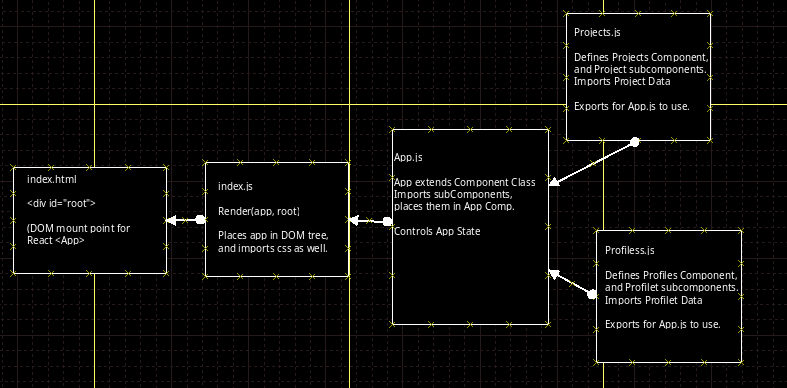
\includegraphics[scale=0.5]{appstructure.png}


\section*{Breaking Down React: React and Web Development:}

\subsection{}

\subsubsection{}

\begin{itemize}
\item For this section, we will not use the template \textit{create-react-app}, and build a bottom up example.
\item In the end, much of the structure in create-react-app is not necessary to get a minimal example to run.
\item All an app needs is one index.html page, and index.js page.
\item You don't even need to run "npm start" or "node react" - you can use CDNs to load React and ReactDOM libriaries straight into the browser.
\item The Minimal Example is as follows:

\mitem React CDN script tags at the end of index.html
\mitem A div root tag in index.html, so React can insert our <App> into the DOM tree.

In index.js you can just build an app, render() and insert it as normal.

\item
\item
\item
\item
\item
\item
\item
\item
\item
\item
\end{itemize}

\section{}

\subsection{}

\subsubsection{}

\begin{itemize}
\item
\item
\item
\item
\item
\item
\item
\item
\item
\item
\item
\item
\item
\item
\item
\item
\item
\end{itemize}

\section{}

\subsection{}

\subsubsection{}

\begin{itemize}
\item
\item
\item
\item
\item
\item
\item
\item
\item
\item
\item
\item
\item
\item
\item
\item
\item
\end{itemize}

\section{}

\subsection{}

\subsubsection{}

\begin{itemize}
\item
\item
\item
\item
\item
\item
\item
\item
\item
\item
\item
\item
\item
\item
\item
\item
\item
\end{itemize}

\section{}

\subsection{}

\subsubsection{}

\begin{itemize}
\item
\item
\item
\item
\item
\item
\item
\item
\item
\item
\item
\item
\item
\item
\item
\item
\item
\end{itemize}

\section{}

\subsection{}

\subsubsection{}

\begin{itemize}
\item
\item
\item
\item
\item
\item
\item
\item
\item
\item
\item
\item
\item
\item
\item
\item
\item
\end{itemize}

\section{}

\subsection{}

\subsubsection{}

\begin{itemize}
\item
\item
\item
\item
\item
\item
\item
\item
\item
\item
\item
\item
\item
\item
\item
\item
\item
\end{itemize}

\section{}

\subsection{}

\subsubsection{}

\begin{itemize}
\item
\item
\item
\item
\item
\item
\item
\item
\item
\item
\item
\item
\item
\item
\item
\item
\item
\end{itemize}

\section{}

\subsection{}

\subsubsection{}

\begin{itemize}
\item
\item
\item
\item
\item
\item
\item
\item
\item
\item
\item
\item
\item
\item
\item
\item
\item
\end{itemize}

\section{}

\subsection{}

\subsubsection{}

\begin{itemize}
\item
\item
\item
\item
\item
\item
\item
\item
\item
\item
\item
\item
\item
\item
\item
\item
\item
\end{itemize}

\section{}

\subsection{}

\subsubsection{}

\begin{itemize}
\item
\item
\item
\item
\item
\item
\item
\item
\item
\item
\item
\item
\item
\item
\item
\item
\item
\end{itemize}

\section{}

\subsection{}

\subsubsection{}

\begin{itemize}
\item
\item
\item
\item
\item
\item
\item
\item
\item
\item
\item
\item
\item
\item
\item
\item
\item
\end{itemize}

\section{}

\subsection{}

\subsubsection{}

\begin{itemize}
\item
\item
\item
\item
\item
\item
\item
\item
\item
\item
\item
\item
\item
\item
\item
\item
\item
\end{itemize}

\section{}

\subsection{}

\subsubsection{}

\begin{itemize}
\item
\item
\item
\item
\item
\item
\item
\item
\item
\item
\item
\item
\item
\item
\item
\item
\item
\end{itemize}


\begin{thebibliography}{9}

\bibitem{ganacheSE}
\url{https://ethereum.stackexchange.com/questions/109847/how-to-install-ganache-ui-on-ubuntu-20-04-lts}
\bibitem{}
\url{}
\bibitem{}
\url{}
\bibitem{}
\url{}
\bibitem{}
\url{}
\bibitem{}
\url{}

	
\end{thebibliography}


\end{document}
